\begin{tikzpicture}
\node[anchor=north west] (int) at (0,0) {
    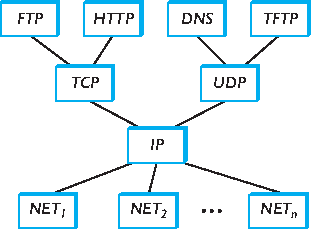
\includegraphics[height=0.75\mypaperheight]{../intro/systemsapproach-1-fig-14.pdf}
};
%\draw[help lines] (0, 0) grid (14, -8);
%\draw[step=2,draw,thick,red] (0, 0) grid (14, -8);
\tikzset{
    layer hi/.style={draw=red,ultra thick},
    layer label/.style={anchor=west},
}
\draw[layer hi] (0, 0) rectangle (9, -1.3);
\node[layer label] at (9.1, -0.65) { application {\it\small OSI layer 7} };
\draw[layer hi] (1.5, -1.8) rectangle (7.5, -3.2);
\node[layer label] at (8.6, -2.5) { transport {\it\small OSI layer 4} };
\draw[layer hi,alt=<2>{fill=red,fill opacity=0.1}] (3.5, -3.6) rectangle (5.6, -4.85);
\node[layer label] at (5.8, -4.2) (net label) { network {\it\small OSI layer 3} };
\draw[layer hi] (0.5, -5.5) rectangle (9, -6.6);
\node[layer label] at (9.1, -6) { data link {\it\small OSI layer 2} };
\begin{visibleenv}<2>
    \node[anchor=west,red,font=\large] at (net label.east) {``narrow waist''};
\end{visibleenv}
\end{tikzpicture}